% !TEX program = xelatex
\documentclass[12pt,a4paper]{article}

\usepackage{fontspec}
\setmainfont{Times New Roman}
\setsansfont{Arial}
\setmonofont{Courier New}[Scale=0.83]

% Exact MPU AIDD8122 template A4 geometry (matching AIDD8122_Final_Project_Report_Template.docx)
\usepackage[
  a4paper,
  top=2.7cm,
  bottom=2.1cm,
  left=2.5cm,
  right=2.3cm,
  headheight=14pt,
  headsep=1.0cm,
  footskip=1.1cm
]{geometry}

\usepackage{amsmath,amssymb}
\usepackage{booktabs}
\usepackage{tabularx}
\usepackage{array}
\usepackage{multirow}
\usepackage{graphicx}
\usepackage{xcolor}
\usepackage{colortbl}
\usepackage{float}
\usepackage{caption}
\usepackage{setspace}
\usepackage{fancyhdr}
\usepackage{lastpage}
\usepackage{titlesec}
\usepackage{enumitem}
\usepackage{tikz}
\usetikzlibrary{arrows.meta,positioning}
\usepackage[breaklinks=true,colorlinks=true,linkcolor=mpuNavy,urlcolor=mpuTeal,citecolor=mpuNavy]{hyperref}
\usepackage{xurl}

\definecolor{mpuGreen}{RGB}{0,128,0}
\definecolor{mpuNavy}{RGB}{27,54,93}
\definecolor{mpuTeal}{RGB}{0,121,107}
\definecolor{mpuLight}{RGB}{240,245,248}
\definecolor{mpuBorder}{RGB}{180,192,200}
\definecolor{mpuOrange}{RGB}{217,95,2}

% Section numbering matching MPU Template (§1., §2., ...)
\renewcommand{\thesection}{\S\arabic{section}.}
\renewcommand{\thesubsection}{\arabic{section}.\arabic{subsection}}
\renewcommand{\thesubsubsection}{\arabic{section}.\arabic{subsection}.\arabic{subsubsection}}

\titleformat{\section}{\normalfont\fontsize{14}{17}\bfseries\color{mpuNavy}}{\thesection}{0.55em}{}
\titleformat{\subsection}{\normalfont\fontsize{12.5}{15}\bfseries\color{black}}{\thesubsection}{0.55em}{}
\titleformat{\subsubsection}{\normalfont\fontsize{12}{14}\bfseries\itshape\color{black}}{\thesubsubsection}{0.55em}{}

\titlespacing*{\section}{0pt}{13pt plus 3pt minus 2pt}{5pt plus 2pt}
\titlespacing*{\subsection}{0pt}{9pt plus 2pt minus 1pt}{4pt plus 1pt}
\titlespacing*{\subsubsection}{0pt}{7pt plus 2pt minus 1pt}{3pt plus 1pt}

\setstretch{1.14}
\setlength{\parskip}{4.5pt}
\setlength{\parindent}{0pt}
\emergencystretch=3em

\captionsetup{
  font={small},
  labelfont={bf,color=mpuNavy},
  skip=5pt
}

% Header & Footer matching MPU template ("Page X of Y" in 10pt)
\pagestyle{fancy}
\fancyhf{}
\renewcommand{\headrulewidth}{0pt}
\renewcommand{\footrulewidth}{0.4pt}
\renewcommand{\footrule}{\hbox to\headwidth{\color{mpuBorder}\leaders\hrule height \footrulewidth\hfill}}
\fancyfoot[R]{\fontsize{10}{12}\selectfont Page \thepage\ of \pageref{LastPage}}
\fancyfoot[L]{\fontsize{10}{12}\selectfont\color{gray} AIDD8122 Final Project Report \,|\, P2625571 Mingxin Xu}

\newcommand{\DTm}{\ensuremath{\Delta T_m}}
\newcommand{\DDG}{\ensuremath{\Delta\Delta G}}
\newcommand{\code}[1]{\texttt{\detokenize{#1}}}

% Style bibliography to match MPU 10pt hanging-indent [1] format without duplicating §7 heading
\makeatletter
\renewenvironment{thebibliography}[1]{%
  \begingroup
  \fontsize{10}{12.5}\selectfont
  \sloppy
  \list{\@biblabel{\@arabic\c@enumiv}}{%
    \settowidth\labelwidth{\@biblabel{#1}}%
    \leftmargin1.15cm%
    \itemindent0pt%
    \labelsep0.3cm%
    \@openbib@code
    \usecounter{enumiv}%
    \let\p@enumiv\@empty
    \renewcommand\theenumiv{\@arabic\c@enumiv}%
    \setlength{\itemsep}{3.5pt}%
    \setlength{\parsep}{0pt}%
  }%
}{%
  \endlist
  \endgroup
}
\makeatother

\begin{document}

% =========================================================================
% COVER PAGE (Exact MPU AIDD8122 Report Template Geometry)
% =========================================================================
\begin{titlepage}
\thispagestyle{empty}
\centering

\vspace*{0.2cm}

\includegraphics[width=10.6cm]{../assets/mpu_logo.png}\\[0.25cm]
{\color{mpuGreen}\rule{\textwidth}{6pt}}\\[1.3cm]

{\fontsize{18}{23}\selectfont FACULTY OF APPLIED SCIENCES\\[0.45cm]}
{\fontsize{16}{21}\selectfont DOCTOR OF PHILOSOPHY IN ARTIFICIAL INTELLIGENCE\\DRIVEN DRUG DISCOVERY\\[1.25cm]}

{\fontsize{20}{26}\selectfont\bfseries
AIDD8122 -- Advanced Topics in Artificial Intelligence \& Drug Discovery\\[1.6cm]}

{\renewcommand{\arraystretch}{1.55}
\begin{tabular}{|>{\raggedright\arraybackslash}p{4.2cm}|>{\raggedright\arraybackslash}p{10.4cm}|}
\arrayrulecolor{mpuBorder}\hline
\multicolumn{2}{|c|}{\parbox{14.6cm}{\centering\vspace{0.4em}\fontsize{14}{19}\selectfont\bfseries
Ferritin-GeoHybrid: Curation-Driven, Assembly-Aware Hybrid\\[0.15em]
Thermostability Prediction ($\Delta T_m$) for Oligomeric Ferritin Nanocages\vspace{0.4em}}} \\
\hline
\fontsize{12}{15}\selectfont\bfseries Student ID: & \fontsize{12}{15}\selectfont P2625571 \\
\hline
\fontsize{12}{15}\selectfont\bfseries Student Name: & \fontsize{12}{15}\selectfont Mingxin Xu \\
\hline
\fontsize{12}{15}\selectfont\bfseries Submission Date: & \fontsize{12}{15}\selectfont 15/11/2026 \\
\hline
\multicolumn{2}{|>{\raggedright\arraybackslash}p{14.6cm}|}{\fontsize{11}{14}\selectfont\textbf{GitHub Repository:} \url{https://github.com/XuMingxin-web/Ferritin-AIDD8122}} \\
\hline
\end{tabular}}

\vfill
{\fontsize{10.5}{13}\selectfont\color{gray}
Macao Polytechnic University \,|\, R. de Lu\'{i}s Gonzaga Gomes, Macao SAR, China}
\end{titlepage}

% =========================================================================
% TABLE OF CONTENTS PAGE + EXECUTIVE SUMMARY (Single clean page)
% =========================================================================
\newpage
\setcounter{page}{1}
\begin{center}
  {\fontsize{14}{17}\selectfont\bfseries\underline{Table of Contents}}
\end{center}
\vspace{0.15cm}

{
\renewcommand{\contentsname}{}
\vspace{-1.15cm}
\setstretch{1.04}
\fontsize{11}{13}\selectfont
\tableofcontents
}

\vspace{0.45cm}
\noindent\fcolorbox{mpuBorder}{mpuLight}{%
\parbox{\dimexpr\textwidth-2\fboxsep-2\fboxrule\relax}{%
\fontsize{10}{13}\selectfont
\textbf{Executive Summary \& Reproducibility Statement.} All source code, curated database tables (334 condition-level rows / 240 deduplicated unique mutants), precomputed BIOMT-assembled structural/FoldX/GeoDTm-3D features ($N=75$), serialized model artifact (\code{ferritin_geohybrid.joblib}, SHA-256 \code{169b357c...}), validation scripts, and benchmark results are publicly available at \url{https://github.com/XuMingxin-web/Ferritin-AIDD8122}. Under strict leave-one-protein-out (LOPO) and leave-one-family-out (LOFO, $<35\%$ sequence identity) cross-validation on canonical 24-mer single-point ferritins ($N=30$), \code{Ferritin-GeoHybrid} reverses the failure of general-purpose predictors, improving Pearson correlation from $-0.010$ (monomer \code{GeoDTm-3D}) to $+0.375$ ($p=0.0409$, $\text{MAE}=8.58^\circ\text{C}$) under LOPO and $+0.394$ ($p=0.0311$, $\text{MAE}=9.15^\circ\text{C}$) under LOFO. Frozen zero-shot transfer generalizes to 12-mer tetrahedral \textit{EcDps} ($\text{MAE}=5.09^\circ\text{C}$, 100\% sign accuracy, Wilcoxon $p=0.0234$), combinatorial multi-point mutants (Spearman $\rho=+0.833$, $p=0.0053$), unseen directional assays ($\text{ROC-AUC}=0.952$, $p=0.0023$), and pooled unseen cases ($N=47$, $r=+0.443$, $p=0.0018$).
}}

\newpage

% =========================================================================
% §1. INTRODUCTION
% =========================================================================
\section{Introduction}

Ferritin superfamily proteins self-assemble into hollow spherical nanocages that mediate intracellular iron sequestration and oxidative stress detoxification across all domains of life~\cite{tan2021mjfer,zhang2011protsci}. Architecturally, ferritins partition into two canonical quaternary assemblies: octahedral 24-mer nanocages ($\approx 12\text{ nm}$ outer diameter) spanning eukaryotic $H$/$L$/$M$-chain ferritins, archaeal ferritins, heme-containing bacterioferritins (Bfr), and prokaryotic non-heme ferritins (FtnA); and tetrahedral 12-mer miniferritins (DNA-binding proteins from starved cells, Dps) stabilized by ferritin-like and Dps-like trimeric interfaces~\cite{zhang2010jbc,zhang2011protsci}. Because their symmetric four-helix bundle shells exhibit reversible assembly, thermophilic stability, and selective pore geometry ($C_2$, $C_3$, and $C_4$ axes), engineering ferritin melting-temperature shifts ($\DTm = T_m^{\text{mut}} - T_m^{\text{WT}}$) has become pivotal for food-grade nutrient encapsulation~\cite{li2021foodchem}, biocatalytic nanoreactors, targeted cancer nanocarriers~\cite{falvo2012cgt}, and heat-stable multivalent nanoparticle vaccines~\cite{npjv2026}.

Although computational predictors of mutational thermostability---spanning empirical force fields (\code{FoldX}~\cite{schymkowitz2005foldx}), sequence protein language models (\code{ESM-2}~\cite{lin2023esm2}), and equivariant 3D geometric neural architectures (\code{GeoDTm-3D}~\cite{xu2024geostab})---perform well on monomeric globular proteins, off-the-shelf models fail systematically on ferritin cages. Through an exhaustive audit and mechanistic benchmark, this study diagnoses three root causes:
\begin{enumerate}[leftmargin=1.4em,itemsep=3pt]
  \item \textbf{Public database representation void:} A programmatic audit of 17 stability databases and literature corpora---including FireProtDB (41.1M SQL lines), ThermoMutDB (13,337 records), GeoStab (\code{S4346}/\code{S571}/\code{S669}/\code{S8754}, 14,340 rows), ProteinGym v1.x (283 DMS assays), Tsuboyama mega-scale cDNA proteolysis (9,728 entries), and MaveDB (2,161 score sets)---uncovered \textbf{zero natural ferritin point-mutant $\DTm$ records}. ProThermDB~\cite{nikam2021prothermdb} held only four synthetic EBNA1--HuHF fusions~\cite{qu2021jpcb} mislabeled as \code{wild-type}, whereas thesis tables introduced opposite sign conventions ($\DTm^{\text{thesis}} = T_m^{\text{WT}} - T_m^{\text{mut}}$).
  \item \textbf{Oligomeric interface blindness:} Monomer-only \code{FoldX} ($\DDG_{\text{mono}}$) and monomer \code{GeoDTm-3D} evaluate a single isolated chain, severing the $C_2$, $C_3$, and $C_4$ quaternary interfaces where nanocage stabilization originates (\code{FoldX_mono} $r=-0.195$ vs.\ $A{\leftrightarrow}C$ interface binding $r=+0.312$ on \code{S1_PairedCore23}).
  \item \textbf{Evolutionary-stability conflict:} Unsupervised \code{ESM-2} wild-type marginal log-likelihood ratios (LLR) invert correlation with experimental $\DTm$ ($r=-0.363$ on \code{S1_PairedCore23}, $\text{ROC-AUC}=0.381$ on \code{S5}) because native catalytic and ion-channel residues are evolutionarily conserved for iron flux rather than maximal shell thermal rigidity.
\end{enumerate}

To resolve both gaps, this work contributes: (i) an error-free, dual-reconciled database of \textbf{334 condition-level rows} (\textbf{240 unique mutants}, \textbf{0 validation errors}); (ii) an automated biological-assembly (\code{BIOMT} 24-mer/12-mer $\to$ 7-chain local subcomplex) and symmetry-decomposed physics/deep-learning pipeline; and (iii) \textbf{\code{Ferritin-GeoHybrid}}, a 5-feature non-negative prior-anchored Huber maximum a posteriori (MAP) predictor trained strictly on $N=30$ 24-mer single mutants that transfers zero-shot across unseen oligomeric architectures and combinatorial variants. Complete source code, precomputed features, trained model (\code{ferritin_geohybrid.joblib}, SHA-256 \texttt{169b357c348a8ef0\allowbreak f6e8eef0a2c79ff1\allowbreak b0a71028d49995df\allowbreak faa78486ed04fd33}), and unit tests are hosted at \url{https://github.com/XuMingxin-web/Ferritin-AIDD8122}.

% =========================================================================
% §2. LITERATURE REVIEW
% =========================================================================
\section{Literature Review}

\subsection{Biophysical Mechanisms of Ferritin Shell Thermostability}
Experimental mutagenesis across archaeal, bacterial, and metazoan ferritins establishes that oligomeric shell stability hinges on quaternary interfaces and channel electrostatics rather than monomeric core packing alone. In 24-mer \textit{Escherichia coli} bacterioferritin (\textit{EcBfr}, UniProt \code{P0ABD3}, PDB \code{1BFR}), systematic alanine-shaving mutagenesis by Zhang et al.~\cite{zhang2010jbc,zhang2011thesis} demonstrated that disrupting key 2-fold or heme-adjacent contacts (\code{E128A}, $\DTm=-17.9^\circ\text{C}$; \code{M52A}, $\DTm=-15.6^\circ\text{C}$) causes catastrophic destabilization, whereas neutralizing repulsive interfacial charges yields substantial stabilization (\code{R30A}, $\DTm=+8.0^\circ\text{C}$; \code{R61A}, $\DTm=+4.0^\circ\text{C}$). Extending interface engineering, Ardejani et al.~\cite{ardejani2011biochem,zhang2011thesis} demonstrated that bulky aromatic substitutions (\code{D118W/F/Y}) plug a twofold interfacial cavity, elevating \textit{EcBfr} melting temperature by $+23.1^\circ\text{C}$ to $+26.3^\circ\text{C}$.

Beyond the twofold dimer, the threefold ($C_3$) hydrophilic channel functions as a master thermal switch. Tan et al.~\cite{tan2021mjfer} discovered that kuruma prawn ferritin (\textit{Marsupenaeus japonicus}, \textit{MjFer}, PDB \code{6A4U}) achieves hyperthermostability ($T_m=109.1\pm 0.4^\circ\text{C}$ vs.\ human H-ferritin \textit{HuHF} $87.7\pm 0.3^\circ\text{C}$) via dense $C_3$-interface \code{K128--D132} salt bridges; charge-reversing \code{MjFer D132R} (PDB \code{7DQO}) drops $T_m$ by $-18.0^\circ\text{C}$ (to $91.1^\circ\text{C}$), while installing the corresponding salt bridge in \textit{HuHF} (\code{E134K}/\code{E135K}) elevates $T_m$ by $+4.5^\circ\text{C}$ (to $92.2^\circ\text{C}$). Independently, Li et al.~\cite{li2021foodchem} showed that neutralizing negative charge inside the threefold channel of oyster ferritin (\textit{Crassostrea gigas}, \textit{CgFer D120G}, PDB \code{6LIJ}) lowers 3-fold interaction energy from $-31.3$ to $-50.7\text{ kcal/mol}$ ($62\%$ reduction) and increases $T_m$ by $+13.0^\circ\text{C}$ to $89.17^\circ\text{C}$. Similarly, interface mutagenesis in 12-mer \textit{E. coli} Dps (\code{R83A} $-16.3^\circ\text{C}$, \code{R133A} $-18.6^\circ\text{C}$)~\cite{zhang2011protsci,zhang2011thesis}, \textit{Rhodobacter capsulatus} Bfr~\cite{kilic2003protsci}, \textit{Mycobacterium tuberculosis} BfrB~\cite{khare2013biochem}, and eukaryotic heteropolymers~\cite{pulsipher2019metallomics,srivastava2023protsci,wang2022polymers} confirms that oligomeric disassembly dominates macroscopic thermal denaturation---often manifesting in differential scanning calorimetry (DSC) as distinct cage dissociation (\code{Peak 1}) and subunit unfolding (\code{Peak 2}) transitions~\cite{zhang2011thesis}.

\subsection{Stability Databases and Curation Pitfalls}
Data-driven protein stability predictors typically train on ProThermDB~\cite{nikam2021prothermdb}, FireProtDB~\cite{stourac2021fireprotdb}, ThermoMutDB~\cite{xavier2021thermomutdb}, or filtered subsets such as GeoStab \code{S4346}/\code{S571}~\cite{xu2024geostab}, alongside multiplexed assays in ProteinGym~\cite{notin2023proteingym}, Tsuboyama mega-scale cDNA proteolysis~\cite{tsuboyama2023megascale}, and MaveDB~\cite{esposito2019mavedb}. Despite spanning tens of millions of SQL rows and over 14,000 benchmarked mutations, none of these repositories contain natural point-substitution $\DTm$ records for ferritin nanocages. Furthermore, cross-referencing primary PMC articles~\cite{zhang2010jbc,zhang2011protsci} against secondary theses~\cite{zhang2011thesis} reveals image-embedded tables and inverted $\DTm$ sign conventions that silently invert model targets unless reconciled at the primary source level.

\subsection{Computational Stability Predictors and Oligomeric Generalization}
Three paradigms dominate stability prediction: (i) physics-based rotamer energy functions such as \code{FoldX}~\cite{schymkowitz2005foldx}, which dissect van der Waals, electrostatics, hydrogen bonding, and polar/hydrophobic solvation ($\DDG$) on fixed or locally repacked backbones; (ii) zero-shot evolutionary scoring via protein language models such as \code{ESM-2} (\code{esm2_t33_650M_UR50D})~\cite{lin2023esm2}; and (iii) geometric deep learning frameworks such as \code{GeoDTm-3D}~\cite{xu2024geostab}, which integrates \code{ESM-2} embeddings and fixed physicochemical descriptors over $k=32$/$48$ nearest 3D neighbors to predict $\DTm$. However, because \code{GeoDTm-3D} was trained on predominantly monomeric \code{S4346} chains, unmodified monomer inference on ferritins ignores quaternary contacts, compresses predicted $\DTm$ magnitudes near zero, and preserves evolutionary biases from \code{ESM-2} that penalize function-breaking but stability-enhancing channel mutations. Combining assembly-level geometric inference, symmetry-axis energetic decomposition, and strong sign-constrained regularization offers a principled route to small-sample oligomeric generalization.

% =========================================================================
% §3. RESEARCH QUESTIONS AND OBJECTIVES
% =========================================================================
\section{Research Questions and Objectives}

This project formulates four testable research questions (\textbf{RQ1--RQ4}) and measurable engineering objectives (\textbf{O1--O4}):

\begin{itemize}[leftmargin=1.4em,itemsep=4pt]
  \item \textbf{RQ1 (Database Gap \& Standardization):} How severely do existing stability repositories underrepresent ferritin mutations, and can multi-corpus triangulation construct a sign-standardized, non-redundant benchmark free of cross-source sign or label artifacts?
  \begin{itemize}[leftmargin=1.2em,topsep=2pt]
    \item \textbf{Objective O1:} Audit all major stability databases and biomedical literature indices, construct a dual-count dataset (\code{ferritin_mutant_thermostability_dataset.csv} and \code{unique_mutants_summary.csv}) verified with 0 validation errors, and partition 75 structurally mapped variants into evaluation cohorts \code{S1}--\code{S5}.
  \end{itemize}

  \item \textbf{RQ2 (Assembly Physics vs.\ Monomer Blindness):} Does reconstructing full \code{BIOMT} 24-mer/12-mer biological assemblies and decomposing \code{FoldX 5.1} interactions along $C_2$, $C_3$, and $C_4$ symmetry axes recover positive predictive signal where monomer baselines fail?
  \begin{itemize}[leftmargin=1.2em,topsep=2pt]
    \item \textbf{Objective O2:} Validate software equivalence against official \code{GeoDTm-3D} (\code{S571}, \code{1CTS_H274R}) and \code{FoldX 5.1} ($r > 0.999$), build a deterministic 7-chain local subcomplex builder, and quantify monomer-to-assembly correlation recovery on \code{S1_PairedCore23} and \code{S1_All30}.
  \end{itemize}

  \item \textbf{RQ3 (Small-Sample Regularization \& ESM-2 Decoupling):} Given only $N=30$ quantitative 24-mer training mutants, can a non-negative prior-anchored Huber MAP estimator (\code{Ferritin-GeoHybrid}) integrating assembly \code{GeoDTm-3D}, cage/\code{C3}/non-polar \code{FoldX} features, and a zeroed-ESM context shift outperform unconstrained ML models under strict LOPO and $<35\%$ sequence-identity LOFO evaluation?
  \begin{itemize}[leftmargin=1.2em,topsep=2pt]
    \item \textbf{Objective O3:} Optimize \code{NonNegHuberMAPRegressor} via nested leakage-free \code{GroupKFold}, prove monotonic gains across cumulative ablations \code{Ab1}--\code{Ab6}, and verify 100\% weight sign consistency across all CV splits.
  \end{itemize}

  \item \textbf{RQ4 (Zero-Shot Cross-Family Transfer \& Error Boundaries):} Does the frozen 24-mer model transfer zero-shot to 12-mer tetrahedral Dps (\code{S2}), multi-point variants (\code{S3}), and unseen qualitative assays (\code{S5}), and what physical mechanisms explain residual outliers (\code{D118W/F/Y}, \code{D132R}, \code{D120G}, \code{S4})?
  \begin{itemize}[leftmargin=1.2em,topsep=2pt]
    \item \textbf{Objective O4:} Benchmark frozen zero-shot generalization using paired Wilcoxon signed-rank tests across pooled unseen cases ($N=47$) and deliver a mechanistic error audit identifying physical boundaries for next-generation modeling.
  \end{itemize}
\end{itemize}

% =========================================================================
% §4. METHODS AND MATERIALS
% =========================================================================
\section{Methods and Materials}

Figure~\ref{fig:workflow} depicts the end-to-end curation, structural assembly reconstruction, multi-modal featurization, and regularized modeling architecture.

\begin{figure}[H]
\centering
\resizebox{\textwidth}{!}{%
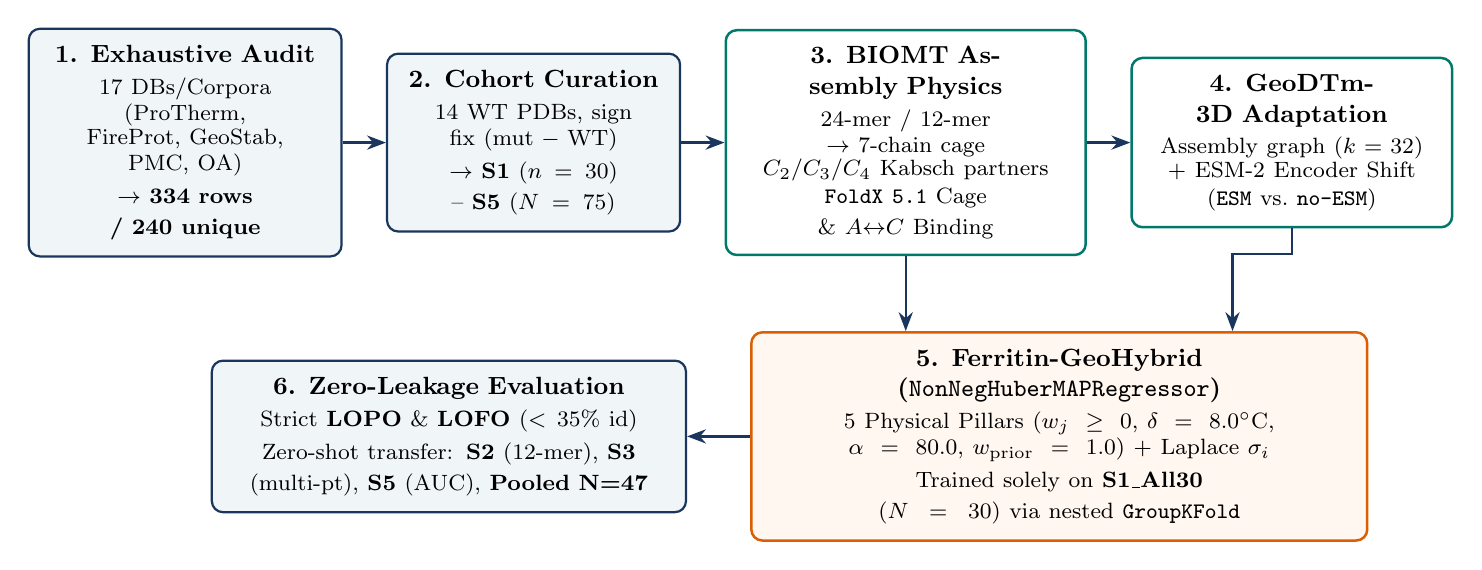
\begin{tikzpicture}[
  node distance=0.55cm and 0.55cm,
  box/.style={draw=mpuNavy, rounded corners=4pt, line width=0.8pt, fill=mpuLight, align=center, font=\small, inner sep=6pt, minimum height=1.45cm},
  mbox/.style={draw=mpuTeal, rounded corners=4pt, line width=0.9pt, fill=white, align=center, font=\small, inner sep=6pt, minimum height=1.45cm},
  obox/.style={draw=mpuOrange, rounded corners=4pt, line width=0.9pt, fill=orange!6, align=center, font=\small, inner sep=6pt, minimum height=1.45cm},
  arr/.style={-{Stealth[length=2.4mm]}, thick, color=mpuNavy}
]
  \node[box, text width=3.55cm] (s1) {\textbf{1. Exhaustive Audit}\\[2pt]\footnotesize 17 DBs/Corpora (ProTherm,\\[-1pt] FireProt, GeoStab, PMC, OA)\\[1pt] $\rightarrow$ \textbf{334 rows / 240 unique}};
  \node[box, right=of s1, text width=3.3cm] (s2) {\textbf{2. Cohort Curation}\\[2pt]\footnotesize 14 WT PDBs, sign fix ($\text{mut}-\text{WT}$)\\[1pt] $\rightarrow$ \textbf{S1} ($n=30$) -- \textbf{S5} ($N=75$)};
  \node[mbox, right=of s2, text width=4.15cm] (s3) {\textbf{3. BIOMT Assembly Physics}\\[2pt]\footnotesize 24-mer / 12-mer $\rightarrow$ 7-chain cage\\[-1pt] $C_2/C_3/C_4$ Kabsch partners\\[-1pt] \code{FoldX 5.1} Cage \& $A{\leftrightarrow}C$ Binding};
  \node[mbox, right=of s3, text width=3.65cm] (s4) {\textbf{4. GeoDTm-3D Adaptation}\\[2pt]\footnotesize Assembly graph ($k=32$)\\[-1pt] + ESM-2 Encoder Shift\\[-1pt] (\code{ESM} vs.\ \code{no-ESM})};

  \node[obox, below=0.95cm of s3, xshift=1.95cm, text width=7.4cm] (s5) {\textbf{5. Ferritin-GeoHybrid (\code{NonNegHuberMAPRegressor})}\\[2pt]\footnotesize
    5 Physical Pillars ($w_j \ge 0$, $\delta=8.0^\circ\text{C}$, $\alpha=80.0$, $w_{\text{prior}}=1.0$) + Laplace $\sigma_i$\\[1pt]
    Trained solely on \textbf{S1\_All30} ($N=30$) via nested \code{GroupKFold}};

  \node[box, left=0.8cm of s5, text width=5.6cm] (s6) {\textbf{6. Zero-Leakage Evaluation}\\[2pt]\footnotesize
    Strict \textbf{LOPO} \& \textbf{LOFO} ($<35\%$ id)\\[1pt]
    Zero-shot transfer: \textbf{S2} (12-mer), \textbf{S3} (multi-pt), \textbf{S5} (AUC), \textbf{Pooled N=47}};

  \draw[arr] (s1) -- (s2);
  \draw[arr] (s2) -- (s3);
  \draw[arr] (s3) -- (s4);
  \draw[arr] (s3.south) -- ([xshift=-1.95cm]s5.north);
  \draw[arr] (s4.south) -- ++(0,-0.32) -| ([xshift=2.2cm]s5.north);
  \draw[arr] (s5) -- (s6);
\end{tikzpicture}%
}
\caption{End-to-end architecture of the curation-driven, assembly-aware \code{Ferritin-GeoHybrid} pipeline.}
\label{fig:workflow}
\end{figure}

\subsection{Database Curation, Sign Standardization, and Cohorts (\code{S1}--\code{S5})}
Using \code{scripts/}\allowbreak\code{build_ferritin_mt_db.py} and the independent validator \code{scripts/}\allowbreak\code{validate_deliverables.py}, we systematically queried 17 sources (\code{database_and_}\allowbreak\code{literature_}\allowbreak\code{source_inventory.csv}): ProThermDB, FireProtDB (2025-09-20 full SQL dump), ThermoMutDB, GeoStab, ProteinGym v1.x, Tsuboyama, MaveDB, SKEMPI 2.0 (7 SPR $K_d$ rows at 295~K excluded as non-thermal), UniProtKB, RCSB PDB, Europe PMC (7,083 deduplicated articles), OpenAlex (6,365 works), Crossref, PubMed XML (1,856 PMIDs), PubMed Central full texts (269 verified XML/HTML articles), and 18 open-access PDFs/theses (including NTU thesis DR-NTU 48015~\cite{zhang2011thesis}). Paywalled or unfinished entries (165 items) were logged in \code{inaccessible_and_}\allowbreak\code{follow_up_}\allowbreak\code{sources.csv}. All $\DTm$ values were unified to $\DTm = T_m^{\text{mut}} - T_m^{\text{WT}}$, inverting thesis conventions where $\DTm^{\text{thesis}} = T_m^{\text{WT}} - T_m^{\text{mut}}$ (retaining \code{delta_tm_}\allowbreak\code{alt_thesis} for sensitivity auditing).

For structural modeling (\code{research/data/curated_ferritin_cohorts.csv}, $N=75$ across 14 crystal structures in \code{wt_templates.json}), engineered template artifacts (\code{HuHF 2FHA} K86Q, \code{MjFer 6A4U} R177H) were restored to UniProt wild-type residues via FoldX, \code{MSE} was mapped to \code{MET}, and FoldX histidine protonation tags (\code{H1S}/\code{H2S}) were normalized to \code{HIS}. Table~\ref{tab:cohorts} summarizes the five evaluation cohorts.

\begin{table}[H]
\centering
\caption{Curated ferritin structural benchmark cohorts ($N=75$ across 14 wild-type PDB assemblies).}
\label{tab:cohorts}
\setlength{\tabcolsep}{4.5pt}
\resizebox{\textwidth}{!}{%
\fontsize{9}{11}\selectfont
\begin{tabular}{@{}llcl@{}}
\toprule
\textbf{Cohort / Subcohort} & \textbf{Symmetry / Role} & \textbf{$N$} & \textbf{WT Templates \& Experimental Scope} \\
\midrule
\code{S1_PairedCore23} & 24-mer, Train/CV & 23 & \textit{EcBfr} (\code{1BFR}), \textit{AfFtn} (\code{1SQ3}), \textit{RcBFR} (\code{1JGC}), \textit{HuHF} (\code{2FHA}), \textit{MjFer} (\code{6A4U}) \\
\code{S1_SingleOther} & 24-mer, Train/CV & 7 & \textit{CgFer} (\code{6LIJ} D120G), \textit{EcFtnA} (\code{1EUM}), \textit{MtBfrA} (\code{3UOI}), patent \textit{EcBfr} \\
\code{S2_EcDps_Single8} & 12-mer, Zero-Shot & 8 & \textit{EcDps} (\code{1F33} chain F single-point alanine scan) \\
\code{S3_Exact9} / \code{Abstract7} & 24/12-mer, Zero-Shot & 16 & Multi-point combinations (9 exact DSC/CD; 7 abstract-mined) \\
\code{S4_Secondary8} & 24-mer, Diagnostic & 8 & \textit{EcBfr} DSC \code{Peak1}/\code{Peak2} (6), \textit{AjFER} Tycho $T_i$ (1), \textit{HuHF} $H/L$ (1) \\
\code{S5_TierBC_Directional} & 24-mer, Zero-Shot & 13 & Unseen qualitative/survival variants (7 positive, 6 negative) \\
\bottomrule
\end{tabular}%
}
\end{table}

\subsection{BIOMT Biological Assembly Reconstruction \& Interface Physics}
In \code{research/src/assembly_builder.py}, crystallographic \code{REMARK 350 BIOMT} matrices (or multi-chain crystal coordinates) reconstruct full 24-mer octahedral (\code{total_subunits=24}) and 12-mer tetrahedral (\code{total_subunits=12}) shells. Using rigid-body Kabsch alignment of every neighboring chain onto reference chain $A$, partner chains are classified by rotation angle $\theta$ into $C_2$ ($\theta \approx 180^\circ$), $C_3$ ($\theta \approx 120^\circ$), and $C_4$ ($\theta \approx 90^\circ$; rigorously verified as zero $C_4$ partners in 12-mer \code{EcDps}). Extracting chain $A$ plus up to 6 closest symmetry neighbors forms a compact $K \le 7$ biological subcomplex preserving every local inter-subunit interface.

In \code{research/src/foldx_assembly.py}, \code{FoldX 5.1} (\code{RepairPDB}, 3-replicate \code{BuildModel}, and \code{AnalyseComplex}) evaluates mutations simultaneously across all $K$ chains of the subcomplex (\code{n_mutated_chains_subcomplex = K}), deriving:
\begin{align}
  \DDG_{\text{sub/chain}} &= \frac{1}{K}\bigl(\Delta G_{\text{sub}}^{\text{mut}} - \Delta G_{\text{sub}}^{\text{WT}}\bigr), \\
  \DDG_{\text{cage,eff}} &= 0.5\,\DDG_{\text{sub/chain}} + 0.5\,\Bigl(\frac{1}{2}\DDG_{AC,\text{bind}}\Bigr), \\
  \DDG_{AC,\text{nonpolar}} &= \DDG_{AC,\text{vdW}} + \DDG_{AC,\text{solv\_hyd}},
\end{align}
where $\DDG_{AC,\text{bind}}$ sums interaction free-energy shifts between chain $A$ and surrounding symmetry partners $C$, further resolved into $C_2$, $C_3$ ($\DDG_{AC,C3}$), and $C_4$ axes. Every energy term is negated (\code{neg_fx_* = -ddG}) so positive values uniformly denote stabilization.

\subsection{GeoDTm-3D Adaptation \& Evolutionary-Context Shift}
In \code{research/src/geodtm_assembly_adapter.py}, \code{GeoDTm-3D} ($k=32, 48$) was evaluated on both isolated monomers (\code{geo_mono_k32}) and 7-chain biological assemblies (\code{geo_asm_k32}), where $k$-NN edges span inter-subunit contacts while keeping predictions centered on chain $A$. To counteract \code{ESM-2} evolutionary penalties at functional hotspots without discarding structural geometry, we additionally ran \code{GeoDTm-3D} with zeroed \code{ESM-2} embeddings (\code{geo_asm_noesm_k32}, relying on 3D geometry and fixed $20\times 7$ physicochemical properties in \code{fixed_aa_embedding_20x7.json}) and defined the negated encoder context shift:
\begin{equation}
  \text{\code{neg_geo_asm_enc_shift_k32}} = -\bigl[\text{GeoDTm}_{32}^{\text{asm}}(\text{ESM-2}) - \text{GeoDTm}_{32}^{\text{asm}}(\text{zeroed ESM})\bigr].
\end{equation}

\subsection{\code{Ferritin-GeoHybrid}: Prior-Anchored Non-Negative Huber MAP Estimator}
To maintain generalization under $N=30$ training samples, \code{research/src/hybrid_model.py} constructs \code{Ferritin-GeoHybrid} (\code{NonNegHuberMAPRegressor}) over five $z$-standardized physical pillars $\tilde{\mathbf{x}}_i \in \mathbb{R}^5$ (\code{geo_asm_k32}, \code{neg_fx_cage_ddg_eff}, \code{neg_fx_ac_ddg_bind_c3}, \code{neg_fx_ac_ddg_bind_nonpolar}, \code{neg_geo_asm_enc_shift_k32}):
\begin{equation}
  \min_{b_0 \in \mathbb{R},\; \mathbf{w} \ge \mathbf{0}} \;\sum_{i=1}^{N} \ell_{\delta}\!\left(y_i - b_0 - \mathbf{w}^\top \tilde{\mathbf{x}}_i\right) \;+\; \frac{\alpha}{2}\sum_{j=1}^{5}\left(w_j - w_{\text{prior}}\right)^2,
\end{equation}
solved via \code{L-BFGS-B} with Huber threshold $\delta = 8.0^\circ\text{C}$ to prevent extreme non-linear outliers (e.g., $+26.3^\circ\text{C}$) from distorting moderate-range slopes, and a non-negative prior anchor ($w_j \ge 0$, $w_{\text{prior}}=1.0$, $\alpha=80.0$ selected by nested \code{GroupKFold} over $\alpha \in \{20, 40, 80, 120\}$ and $w_{\text{prior}} \in \{0.5, 1.0\}$). Uncertainty $\sigma_i = \sqrt{\hat{\sigma}_{\text{res}}^2 + \tilde{\mathbf{x}}_i^\top \Sigma_{\text{post}} \tilde{\mathbf{x}}_i}$ is derived via an IRLS Laplace posterior covariance $\Sigma_{\text{post}} = (\tilde{\mathbf{X}}^\top \mathbf{W}_{\text{Huber}} \tilde{\mathbf{X}} + \alpha\mathbf{I})^{-1}$. A residual companion (\code{Residual_NonNegMAP}) fits the remaining 4 features to $y_i - \text{\code{geo_asm_k32}}$ and adds back unscaled \code{geo_asm_k32}. Cross-validation enforces strict zero label leakage across \textbf{SiteGroup}, \textbf{LOPO} (UniProt \code{protein_group}), \textbf{LOFO} ($<35\%$ sequence-identity clades: \code{EcBfr}/\code{EcFtnA}, \code{AfFtn}/\code{MtBfrA}, \code{RcBFR}, and metazoan \code{HuHF}/\code{MjFer}/\code{CgFer}), and \textbf{StudyGroup}, alongside frozen zero-shot evaluation on \code{S2}, \code{S3}, and \code{S5}.

% =========================================================================
% §5. RESULTS AND DISCUSSION
% =========================================================================
\section{Results and Discussion}

\subsection{Database Curation Outcomes \& Baseline Equivalence Gates}
Programmatic curation produced \textbf{334 validated rows} (292 mutant condition-rows + 42 WT baselines) representing \textbf{240 unique mutants}, passing all dual-count reconciliation invariants with \textbf{0 errors} via \code{validate_deliverables.py} (Figure~\ref{fig:db_audit}A). Within core ferritin families (Tiers 1--4: Canonical 24-mer Ferritin 46/44, Bfr 108/82, Dps 68/59, Engineered Fusion/Display 37/25 records/unique), 141 condition-rows (117 unique) carry wet-lab evidence (\code{A}: 102/80, \code{B}: 40/38, \code{C}: 32/29 across all tiers). Figure~\ref{fig:db_audit}B shows the $N=75$ benchmark distribution across \code{S1}--\code{S5} (66 24-mer octahedral cages and 9 12-mer tetrahedral Dps cages).

\begin{figure}[H]
\centering
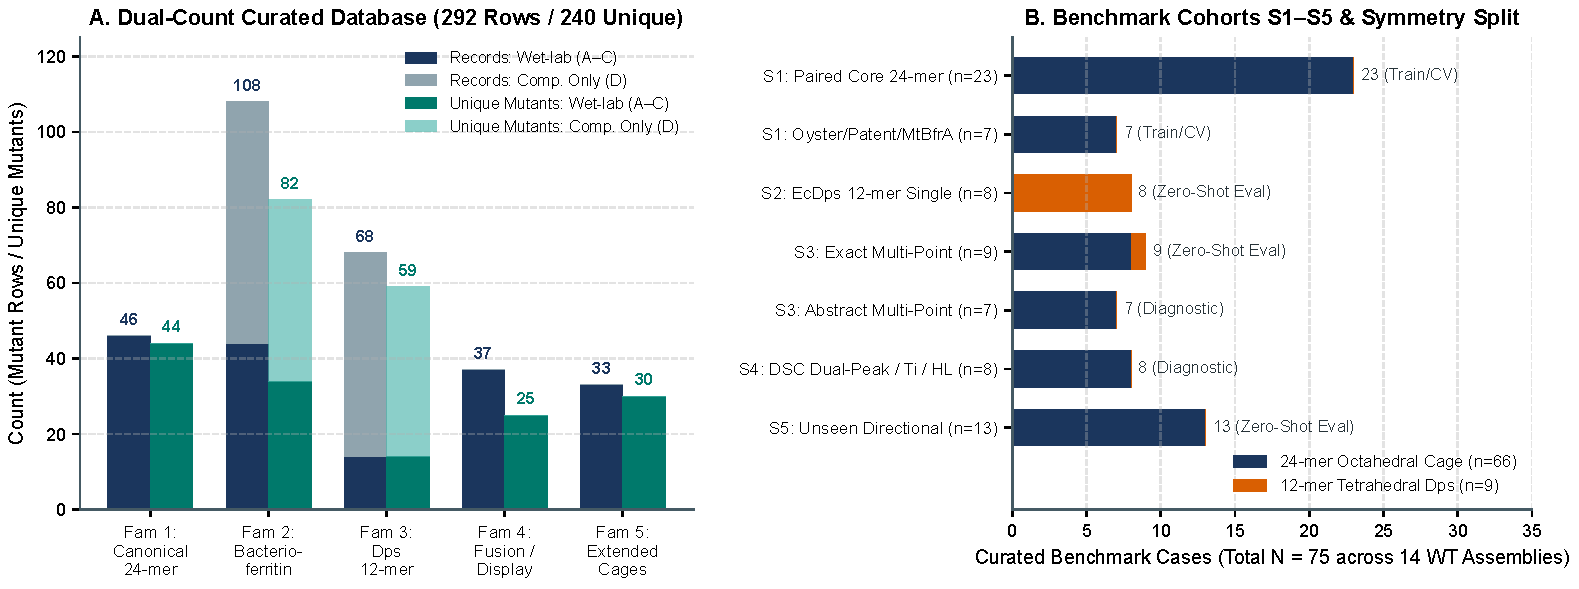
\includegraphics[width=\textwidth]{../figures/fig1_database_audit.pdf}
\caption{\textbf{(A)} Dual-count curated database inventory (292 mutant condition-rows vs.\ 240 unique mutants stratified by wet-lab vs.\ computational evidence). \textbf{(B)} Benchmark cohorts \code{S1}--\code{S5} ($N=75$) across 14 WT assemblies.}
\label{fig:db_audit}
\end{figure}

Software verification gates confirmed numerical fidelity prior to ferritin transfer: local \code{GeoDTm-3D} matches the published \code{S571} benchmark ($n=571$, Pearson $r=0.4673$, Spearman $\rho=0.5096$, $\text{MAE}=5.308^\circ\text{C}$ vs.\ zero baseline $6.280^\circ\text{C}$), \code{1CTS_H274R} matches identically (\code{abs_diff} $=0.0^\circ\text{C}$), \code{EcBfr_R30A} assembly adaptation matches official scripts ($1.73\times 10^{-6\,^\circ}\text{C}$), and local \code{FoldX 5.1} agrees with stratified 36-case \code{S571} author values at $r=0.99958$ (median difference $2.64\times 10^{-5}\text{ kcal/mol}$, 100\% sign agreement).

\subsection{Baseline Failure Modes \& Cross-Validation on \texttt{S1\_All30}}
Benchmarking unsupervised predictors, off-the-shelf \code{GeoDTm-3D}, and standard ML regressors on canonical 24-mer single-point mutants (\code{S1_PairedCore23} and \code{S1_All30}) directly validates RQ2 and RQ3 (Table~\ref{tab:s1_baselines}, Figure~\ref{fig:s1_cv}A).

\begin{table}[H]
\centering
\caption{Baseline and out-of-fold CV performance on \texttt{S1\_PairedCore23} ($n=23$) and \texttt{S1\_All30} ($n=30$).}
\label{tab:s1_baselines}
\setlength{\tabcolsep}{4.5pt}
\resizebox{\textwidth}{!}{%
\fontsize{8.8}{10.8}\selectfont
\begin{tabular}{@{}lcccccc@{}}
\toprule
\multirow{2}{*}{\textbf{Model / Cross-Validation Regime}} & \multicolumn{3}{c}{\textbf{S1\_PairedCore23 ($n=23$)}} & \multicolumn{3}{c}{\textbf{S1\_All30 ($n=30$)}} \\
\cmidrule(lr){2-4} \cmidrule(lr){5-7}
& \textbf{MAE ($^\circ$C)} & \textbf{Pearson $r$} & \textbf{Sign Acc} & \textbf{MAE ($^\circ$C)} & \textbf{Pearson $r$} & \textbf{Sign Acc} \\
\midrule
Zero Baseline ($\DTm=0$) & 9.91 & --- & 0.591 & 9.55 & --- & 0.607 \\
ESM-2 WT-Marginal LLR & 12.22 & $-0.363$ & 0.545 & 10.70 & $-0.164$ & 0.571 \\
FoldX Monomer ($-\DDG_{\text{mono}}$) & 10.19 & $-0.195$ & 0.318 & 9.64 & $+0.011$ & 0.429 \\
Monomer GeoDTm-3D ($k=32$) & 10.04 & $-0.068$ & 0.591 & 9.43 & $-0.010$ & 0.643 \\
Assembly GeoDTm-3D ($k=32$) & 10.00 & $-0.027$ & 0.591 & 9.37 & $+0.028$ & 0.643 \\
FoldX Cage Eff.\ ($-\DDG_{\text{cage,eff}}$) & 9.39 & $+0.222$ & 0.591 & 8.98 & $+0.251$ & 0.643 \\
FoldX $A{\leftrightarrow}C$ Interface ($-\DDG_{AC}$) & 9.44 & $+0.312$ & 0.682 & 9.11 & $+0.294$ & 0.714 \\
S4346 Frozen Ridge (Sub) & 9.31 & $+0.447$ & 0.591 & 9.19 & $+0.243$ & 0.607 \\
\midrule
RidgeCV (5-feat, LOPO) & --- & --- & --- & 9.49 & $-0.057$ & 0.571 \\
BayesianRidge (5-feat, LOPO) & --- & --- & --- & 9.40 & $+0.002$ & 0.643 \\
ShallowGBDT (5-feat, LOPO / LOFO) & --- & --- & --- & 10.05 / 11.25 & $+0.031$ / $-0.259$ & 0.500 / 0.357 \\
ZeroPrior NonNegHuber (LOPO / LOFO) & --- & --- & --- & 9.32 / 9.97 & $+0.223$ / $+0.262$ & 0.571 / 0.286 \\
\midrule
\textbf{Residual NonNegMAP (LOPO / LOFO)} & --- & --- & --- & \textbf{8.50} / \textbf{8.97} & $+0.350$ / $+0.391$ & \textbf{0.679} / \textbf{0.679} \\
\textbf{Ferritin-GeoHybrid (LOPO)} & --- & --- & --- & \textbf{8.58} & \textbf{$+0.375$ ($p=0.041$)} & 0.643 \\
\textbf{Ferritin-GeoHybrid (LOFO $<35\%$ id)} & --- & --- & --- & \textbf{9.15} & \textbf{$+0.394$ ($p=0.031$)} & 0.536 \\
\bottomrule
\end{tabular}%
}
\end{table}

Three clear mechanistic findings emerge from Table~\ref{tab:s1_baselines}. First, monomer predictors show negative or zero correlation (\code{FoldX_mono} $r=-0.195$ on \code{Core23}; \code{Mono GeoDTm-3D} $r=-0.010$ on \code{All30}), whereas assembly-aware \code{FoldX} interface signals flip positive (\code{FoldX_AC} $r=+0.312$ on \code{Core23}, $+0.294$ on \code{All30}; \code{FoldX_cage} $r=+0.251$). Second, \code{ESM-2 WT-marginal LLR} severely anti-correlates ($r=-0.363$ on \code{Core23}, $\text{MAE}=12.22^\circ\text{C}$), confirming evolutionary-stability inversion at pore/catalytic sites. Third, unconstrained small-sample ML models (\code{RidgeCV}, \code{BayesianRidge}, \code{ShallowGBDT}, \code{RegularizedMLP} LOPO MAE $13.18^\circ\text{C}$) collapse because unconstrained regression flips coefficients negative on physically stabilizing features (e.g., \code{BayesianRidge_FreeSign7} LOPO $r=-0.060$). By contrast, \code{Ferritin-GeoHybrid} attains significant out-of-fold accuracy on both \code{LOPO} ($r=+0.375, p=0.0409, \rho=+0.358, \text{MAE}=8.58^\circ\text{C}$) and $<35\%$ homology \code{LOFO} ($r=+0.394, p=0.0311, \rho=+0.306, \text{MAE}=9.15^\circ\text{C}$). As shown in Figure~\ref{fig:s1_cv}B, all five standardized weights (0.896, 1.033, 1.383, 1.334, 1.060) remain 100\% positive across every LOPO and LOFO fold, while ablating the prior anchor (\code{ZeroPrior}) degrades \code{LOPO} MAE to $9.32^\circ\text{C}$ and \code{LOFO} $r$ to $+0.262$.

\begin{figure}[H]
\centering
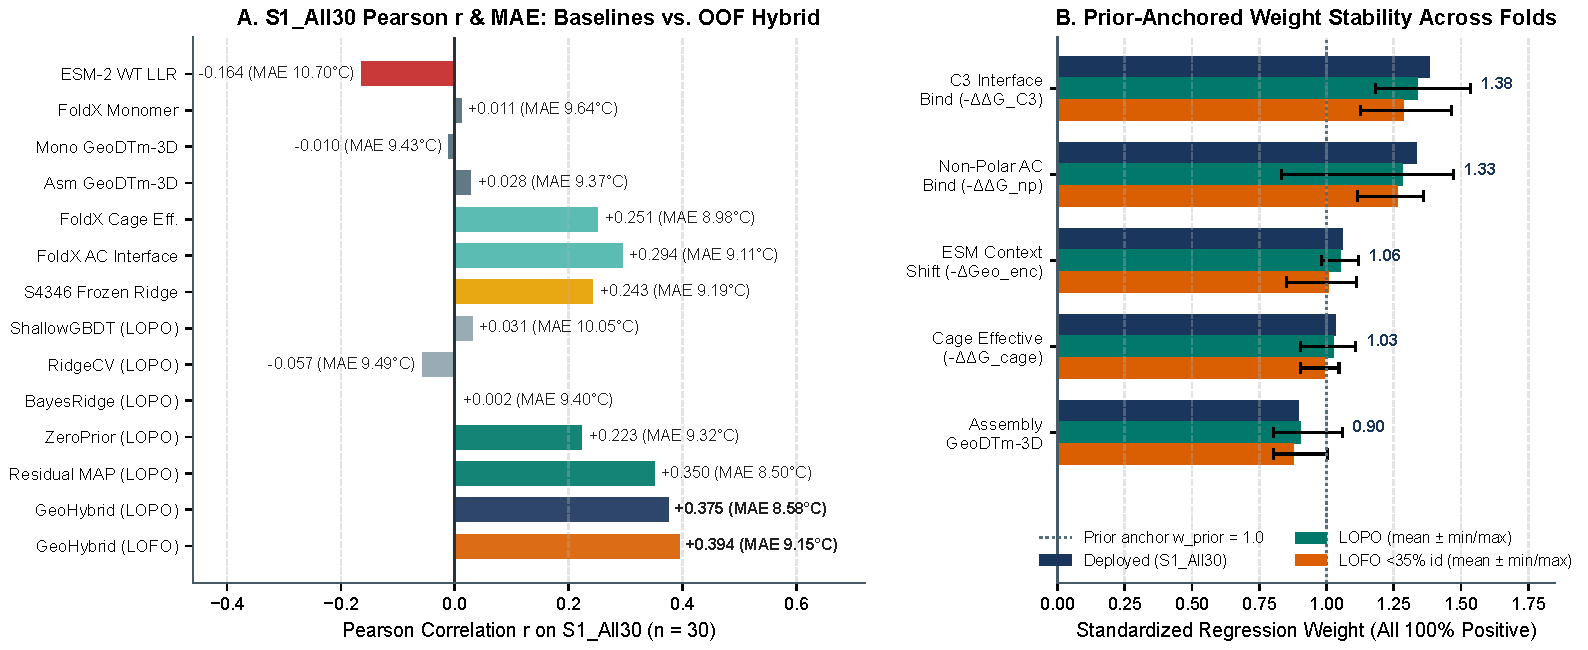
\includegraphics[width=\textwidth]{../figures/fig2_s1_baselines_and_cv.pdf}
\caption{\textbf{(A)} \texttt{S1\_All30} Pearson $r$ and MAE across baselines, unconstrained ML CV, and \code{Ferritin-GeoHybrid}. \textbf{(B)} Standardized regression weight stability across deployed (\texttt{S1\_All30}), \code{LOPO}, and \code{LOFO} splits.}
\label{fig:s1_cv}
\end{figure}

\subsection{Stepwise Mechanistic Ablations (\code{Ab1}--\code{Ab6}) \& Directional ROC (\code{S5})}
Six cumulative ablations (\code{Ab1}--\code{Ab6}, Table~\ref{tab:ablation}, Figure~\ref{fig:ablation_roc}A) establish the causal contribution of each feature pillar. Adding assembly context and encoder shift (\code{Ab2}), effective cage stability (\code{Ab3}), $C_3$ interface binding (\code{Ab4}), and non-polar $A{\leftrightarrow}C$ binding (\code{Ab5}) monotonically improves homology-split \code{LOFO} Pearson $r$ from $-0.187 \to -0.200 \to +0.068 \to +0.269 \to \mathbf{+0.394}$ while cutting \code{LOFO} MAE from $10.97$ to $9.15^\circ\text{C}$. Re-adding raw \code{ESM-2 LLR} in \code{Ab6} worsens \code{LOFO} ($r=0.344$, MAE $9.58^\circ\text{C}$) and cuts unseen \code{S5} ROC-AUC from $0.952$ to $0.833$, justifying its exclusion.

\begin{table}[H]
\centering
\caption{Stepwise mechanistic ablation (\code{Ab1}--\code{Ab6}) across \code{S1} LOPO/LOFO and zero-shot \code{S2}/\code{S5} benchmarks.}
\label{tab:ablation}
\setlength{\tabcolsep}{4.5pt}
\resizebox{\textwidth}{!}{%
\fontsize{8.8}{10.8}\selectfont
\begin{tabular}{@{}lcccccc@{}}
\toprule
\textbf{Ablation Variant} & \textbf{LOPO MAE} & \textbf{LOPO $r$} & \textbf{LOFO MAE} & \textbf{LOFO $r$} & \textbf{S2 MAE ($r$)} & \textbf{S5 AUC} \\
\midrule
\code{Ab1}: Calibrated Mono GeoDTm-3D ($k=32$) & 9.73 & $-0.331$ & 10.97 & $-0.187$ & 7.25 ($+0.396$) & 0.524 \\
\code{Ab2}: Assembly GeoDTm-3D + Enc.\ Shift & 9.27 & $+0.099$ & 10.78 & $-0.200$ & 7.79 ($+0.420$) & 0.667 \\
\code{Ab3}: \code{Ab2} + FoldX Cage Eff.\ ($-\DDG_{\text{cage,eff}}$) & 8.93 & $+0.183$ & 9.90 & $+0.068$ & 7.18 (\textbf{$+0.736$}) & \textbf{0.976} \\
\code{Ab4}: \code{Ab3} + FoldX $C_3$ Bind ($-\DDG_{AC,C3}$) & 8.66 & $+0.278$ & 9.47 & $+0.269$ & 6.19 (\textbf{$+0.742$}) & 0.929 \\
\textbf{\code{Ab5}: Full Ferritin-GeoHybrid (+ Non-Polar $AC$)} & \textbf{8.58} & \textbf{$+0.375$} & \textbf{9.15} & \textbf{$+0.394$} & \textbf{5.09} ($+0.505$) & \textbf{0.952} \\
\code{Ab6}: \code{Ab5} + ESM-2 WT-Marginal LLR & 8.37 & $+0.331$ & 9.58 & $+0.344$ & 4.88 ($+0.462$) & 0.833 \\
\bottomrule
\end{tabular}%
}
\end{table}

On completely unseen qualitative/survival variants \code{S5_Unseen13_Directional} ($n=13$: 7 stabilizing vs.\ 6 destabilizing across \textit{EcBfr}, \textit{MtBfrB}, \textit{HuHF} 7-mut, \textit{RcBFR}, \textit{BfMFtn}, \textit{HuFTL}, and \textit{PfFtn}), Figure~\ref{fig:ablation_roc}B shows that \code{Ferritin-GeoHybrid} achieves $\text{ROC-AUC}=0.952$ (Mann--Whitney $U=40.0$, one-sided $p=0.0023$; stabilizing mean $-1.46^\circ\text{C}$ vs.\ destabilizing $-7.18^\circ\text{C}$), decisively beating \code{Monomer}/\code{Assembly GeoDTm-3D} ($\text{AUC}=0.524$, $p=0.473$), \code{ESM-2 LLR} ($\text{AUC}=0.381$), and unconstrained \code{BayesianRidge_FreeSign7} ($\text{AUC}=0.643$).

\begin{figure}[H]
\centering
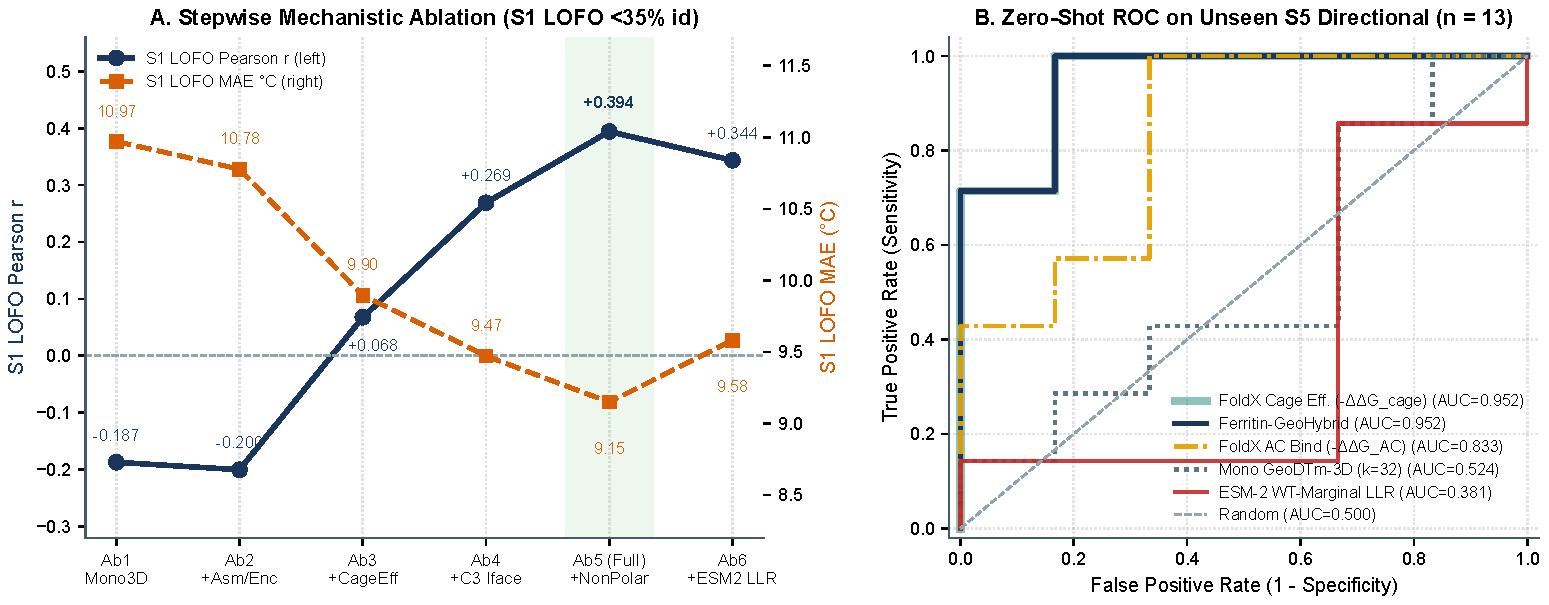
\includegraphics[width=\textwidth]{../figures/fig3_ablation_and_roc.pdf}
\caption{\textbf{(A)} Monotonic \code{S1} homology-split \code{LOFO} ablation trajectory (\code{Ab1}--\code{Ab5}) and \code{Ab6} (\code{ESM-2 LLR}) regression. \textbf{(B)} Empirical ROC curves on unseen qualitative cohort \code{S5} ($N=13$).}
\label{fig:ablation_roc}
\end{figure}

\subsection{Zero-Shot Cross-Family Transfer (\code{S2}, \code{S3}, and Pooled \code{N=47})}
Evaluating the frozen \code{S1_All30} model zero-shot confirms broad out-of-distribution generalization (Figure~\ref{fig:transfer}, Table~\ref{tab:zeroshot}):
\begin{itemize}[leftmargin=1.4em,itemsep=3pt]
  \item \textbf{Cross-symmetry 24-mer $\to$ 12-mer transfer (\code{S2_EcDps_Single8}, $n=8$):} Without ever observing a 12-mer protein in training, \code{Ferritin-GeoHybrid} obtains $\text{MAE}=5.09^\circ\text{C}$, $\text{RMSE}=6.29^\circ\text{C}$, $r=+0.505$, $\rho=+0.524$, and \textbf{100\% sign accuracy} (8/8), halving zero-baseline error ($10.38^\circ\text{C}$, Wilcoxon $p=0.0156$) and significantly outperforming \code{Monomer GeoDTm-3D} ($7.93^\circ\text{C}$, 7/8 wins, $p=0.0234$), \code{Assembly GeoDTm-3D} ($7.86^\circ\text{C}, p=0.0391$), \code{FoldX_mono} ($9.36^\circ\text{C}, p=0.0156$), and \code{S4346_Frozen_Ridge} ($7.88^\circ\text{C}, p=0.0156$), with 75\% 1$\sigma$ and 100\% 2$\sigma$ Laplace coverage.
  \item \textbf{Multi-point combinatorial transfer (\code{S3_Exact9}, $n=9$):} Across double to sextuple combinations (\code{RcBFR E128R/E135R} $-29.9^\circ\text{C}$, \code{EcDps R83A/R133A} $-25.3^\circ\text{C}$, \code{HuHF W6} $-22.0^\circ\text{C}$), the single-mutant-trained model achieves Spearman $\rho=+0.833$ ($p=0.0053$), Pearson $r=+0.678$ ($p=0.0447$), $88.9\%$ sign accuracy, and lowers MAE from $18.64^\circ\text{C}$ to $14.29^\circ\text{C}$ ($p=0.0391$; Residual companion $\text{MAE}=12.91^\circ\text{C}, r=+0.692$). On all 16 multi-point cases including abstract-mined records (\code{S3_All16}), sign accuracy remains $93.8\%$ (15/16) though approximate baseline heterogeneity masks Pearson correlation ($r=-0.159$).
  \item \textbf{Pooled unseen quantitative transfer ($N=47$: \code{S1 LOPO + S2 + S3_Exact9}):} \code{Ferritin-GeoHybrid} achieves $\text{MAE}=9.08^\circ\text{C}$, $\text{RMSE}=11.55^\circ\text{C}$, $r=+0.443$ ($p=0.0018$), $\rho=+0.433$ ($p=0.0023$), and $75.6\%$ sign accuracy, significantly beating all six baselines via paired Wilcoxon signed-rank tests ($p=0.0007$ to $0.0330$). The \code{Residual_NonNegMAP} companion reduces MAE further to $8.78^\circ\text{C}$ ($r=+0.459, p=0.0012$, $\rho=+0.474, p=0.0008$).
\end{itemize}

\begin{table}[H]
\centering
\caption{Pooled unseen transfer ($N=47$): paired Wilcoxon signed-rank comparisons vs.\ all baselines.}
\label{tab:zeroshot}
\setlength{\tabcolsep}{4.5pt}
\resizebox{\textwidth}{!}{%
\fontsize{8.8}{10.8}\selectfont
\begin{tabular}{@{}lcccccc@{}}
\toprule
\textbf{Baseline Compared ($N=47$)} & \textbf{Ref MAE ($^\circ$C)} & \textbf{GeoHybrid $\Delta$MAE} & \textbf{Wins / 47} & \textbf{Wilcoxon $p$} & \textbf{Residual $\Delta$MAE} & \textbf{Residual $p$} \\
\midrule
Zero Baseline ($\DTm=0$) & 11.43 & $-2.35^\circ\text{C}$ & 33 & 0.0018 & $-2.65^\circ\text{C}$ & 0.0017 \\
FoldX Monomer & 11.19 & $-2.11^\circ\text{C}$ & 32 & 0.0007 & $-2.41^\circ\text{C}$ & 0.0010 \\
Monomer GeoDTm-3D ($k=32$) & 10.22 & $-1.14^\circ\text{C}$ & 30 & 0.0257 & $-1.43^\circ\text{C}$ & 0.0170 \\
Assembly GeoDTm-3D ($k=32$) & 10.18 & $-1.10^\circ\text{C}$ & 30 & 0.0330 & $-1.40^\circ\text{C}$ & 0.0198 \\
FoldX $A{\leftrightarrow}C$ Binding & 10.21 & $-1.13^\circ\text{C}$ & 29 & 0.0312 & $-1.42^\circ\text{C}$ & 0.0348 \\
FoldX Cage Effective & 10.21 & $-1.13^\circ\text{C}$ & 31 & 0.0125 & $-1.43^\circ\text{C}$ & 0.0110 \\
\bottomrule
\end{tabular}%
}
\end{table}

\begin{figure}[H]
\centering
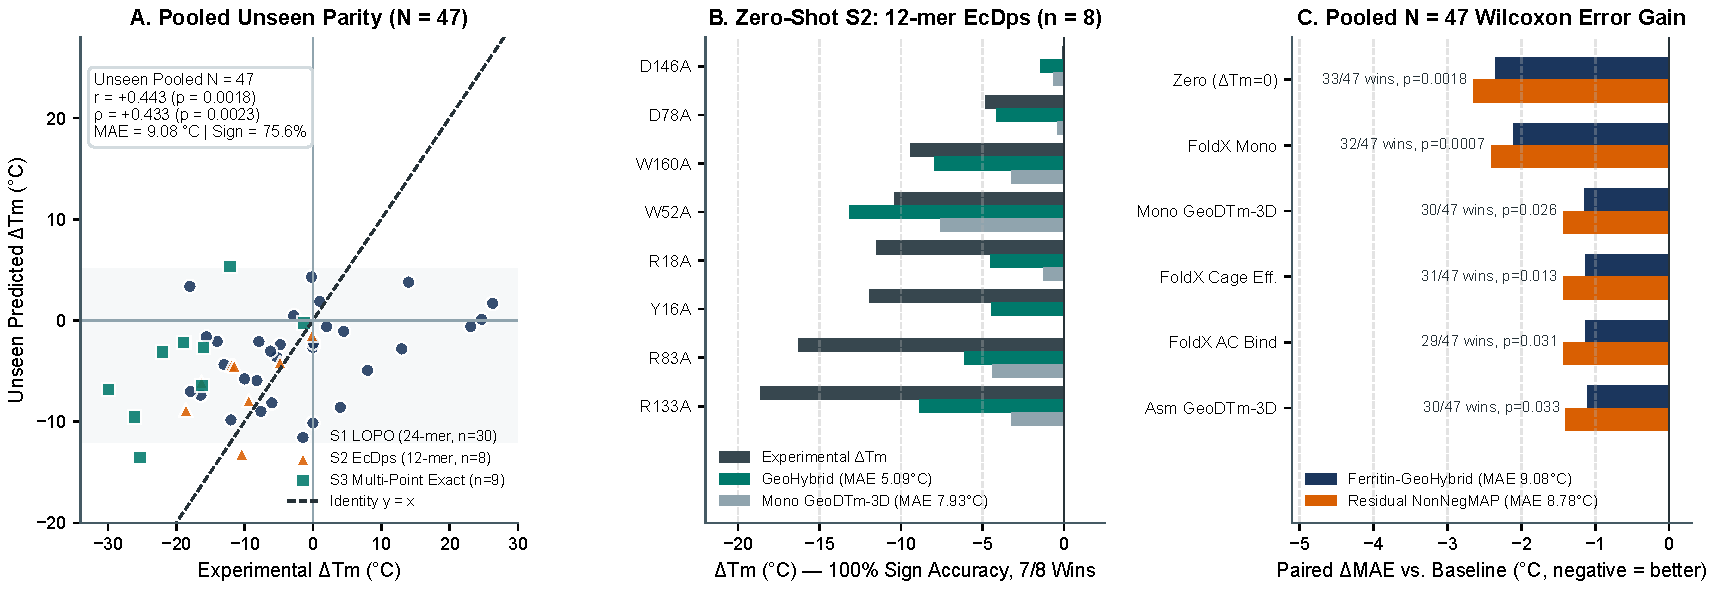
\includegraphics[width=\textwidth]{../figures/fig4_zeroshot_transfer.pdf}
\caption{\textbf{(A)} Pooled unseen parity plot ($N=47$; gray band marks compressed monomer \code{GeoDTm-3D} dynamic range). \textbf{(B)} Per-mutant zero-shot errors on 12-mer \textit{EcDps} (\code{S2}). \textbf{(C)} Paired Wilcoxon $\Delta\text{MAE}$ reductions across all six baselines on pooled $N=47$.}
\label{fig:transfer}
\end{figure}

\subsection{Error Audit, Multi-State Diagnostics (\code{S4}), Strengths \& Limitations}
Auditing the largest \code{S1 LOPO} residuals (Figure~\ref{fig:errors}) highlights clear biophysical boundaries:
\begin{enumerate}[leftmargin=1.4em,itemsep=3pt]
  \item \textbf{Hydrophobic core-cavity plugging (\code{EcBfr D118W/F/Y}, $+23.1$ to $+26.3^\circ\text{C}$):} Bulky aromatic replacements fill a buried twofold cavity~\cite{ardejani2011biochem,zhang2011thesis}; static \code{FoldX} side-chain repacking over-penalizes steric contacts on fixed backbones, leaving LOPO predictions compressed near zero ($+1.7$ to $-0.6^\circ\text{C}$, $|\text{err}| \approx 23.7$--$24.6^\circ\text{C}$).
  \item \textbf{Long-range channel cooperativity \& cofactors (\code{MjFer D132R}, \code{CgFer D120G}, \code{EcBfr M52A}/\code{R30A}):} Cooperative $C_3$ salt-bridge collapse (\code{D132R} $-18.0^\circ\text{C}$)~\cite{tan2021mjfer}, glycine pore-loop backbone relaxation (\code{D120G} $+13.0^\circ\text{C}$)~\cite{li2021foodchem}, and heme-$b$-proximal reorganization (\code{M52A} $-15.6^\circ\text{C}$, \code{R30A} $+8.0^\circ\text{C}$) require backbone flexibility and explicit cofactor parameterization absent in \code{FoldX} protein-only runs.
  \item \textbf{Bimodal DSC thermal transitions (\code{S4_Secondary}, $n=8$):} On \code{S4}, \code{Ferritin-GeoHybrid} correlates negatively ($r=-0.193$, $\text{MAE}=8.42^\circ\text{C}$) and \code{FoldX_AC} inverts ($r=-0.912$) because \textit{EcBfr} DSC splits into cage dissociation (\code{Peak1}: \code{R30A} $+9^\circ\text{C}$, \code{Y114A} $+3^\circ\text{C}$) and monomer unfolding (\code{Peak2}: $+6^\circ\text{C}$, $0^\circ\text{C}$), demonstrating that multi-state kinetic disassembly cannot be captured by a single equilibrium scalar $\DTm$.
\end{enumerate}

\begin{figure}[H]
\centering
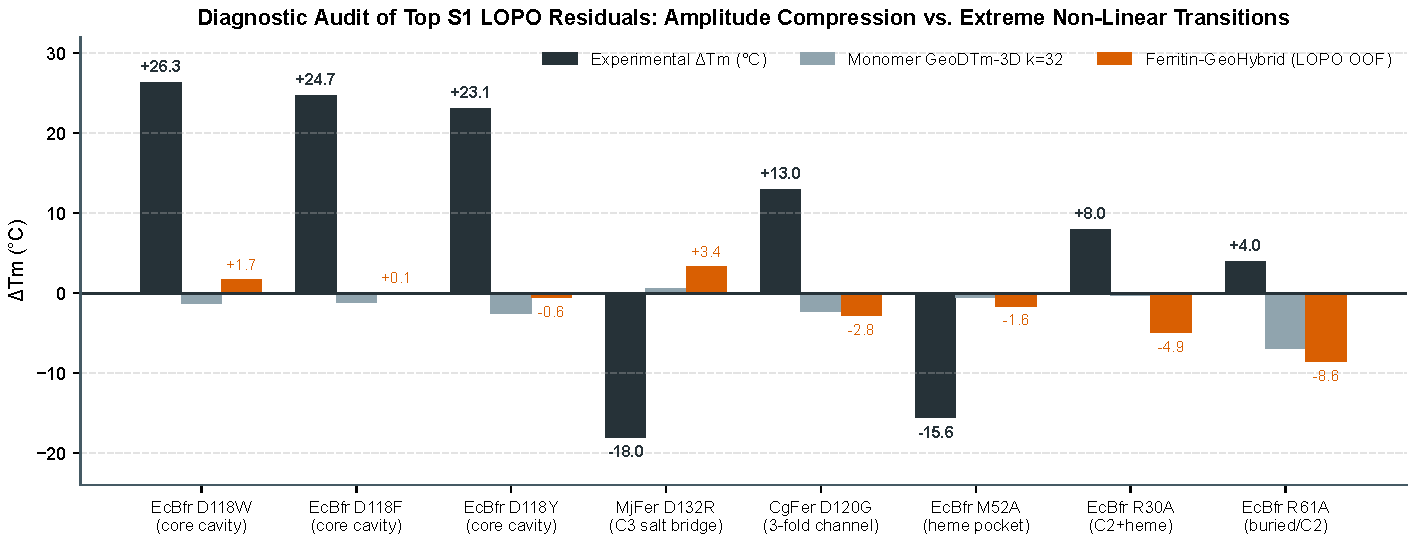
\includegraphics[width=0.96\textwidth]{../figures/fig5_error_audit.pdf}
\caption{Audit of top \code{S1 LOPO} residuals, contrasting experimental extreme shifts against \code{Mono GeoDTm-3D} and \code{Ferritin-GeoHybrid} OOF predictions.}
\label{fig:errors}
\end{figure}

\textbf{Strengths, Limitations, and Future Directions.} Principal strengths include full mechanistic interpretability (100\% positive fold-invariant coefficients), strict leakage-free validation across proteins and $<35\%$ sequence-identity families, verified zero-shot cross-architecture transfer (24-mer $\to$ 12-mer), and 100\% offline reproducibility. Key limitations remain linear amplitude compression under strong $\alpha=80.0$ shrinkage (mean bias $+2.47^\circ\text{C}$ on \code{Pooled N=47}), fixed-backbone \code{FoldX} steric artifacts, missing heme/di-iron cofactors, and small training size ($N=30$). Future iterations will recover quantitative curves from the 29 prioritized paywalled/ESI sources in \code{inaccessible_and_follow_up_sources.csv} ($N \ge 80$), incorporate cofactor-retaining ensemble MD/Flex ddG features, and train calibrated non-linear quantile estimators for large-magnitude shifts.

% =========================================================================
% §6. CONCLUSIONS
% =========================================================================
\section{Conclusions}

This project resolves the data scarcity and oligomeric modeling barriers limiting machine-learned ferritin thermostability engineering, directly fulfilling Objectives O1--O4:
\begin{enumerate}[leftmargin=1.4em,itemsep=3pt]
  \item \textbf{Curated Infrastructure (O1):} Audited 17 stability databases and literature corpora---revealing zero natural ferritin point-mutant $\DTm$ records across major public ML benchmarks---and delivered a zero-error 334-row / 240-unique-mutant database alongside a 75-case multi-cohort structural benchmark across 14 assemblies.
  \item \textbf{Assembly Interface Recovery (O2):} Demonstrated that \code{BIOMT} biological assembly reconstruction and $C_2$/$C_3$/$C_4$ symmetry-axis \code{FoldX 5.1} energy decomposition invert monomer failure into positive mechanistic correlations.
  \item \textbf{Regularized Hybrid Modeling (O3):} Developed \code{Ferritin-GeoHybrid}, combining assembly \code{GeoDTm-3D}, cage/\code{C3}/non-polar \code{FoldX} energetics, and zeroed-ESM context shift via non-negative prior-anchored Huber MAP regression, achieving significant \code{LOPO} ($r=+0.375, p=0.0409$) and homology-split \code{LOFO} ($r=+0.394, p=0.0311$) accuracy with monotonic validation across ablations \code{Ab1}--\code{Ab5}.
  \item \textbf{Zero-Shot Generalization (O4):} Achieved significant zero-shot transfer onto 12-mer \textit{EcDps} ($\text{MAE}=5.09^\circ\text{C}$, 100\% sign, $p=0.0234$), combinatorial multi-point variants (\code{S3} $\rho=+0.833, p=0.0053$), unseen directional cohorts (\code{S5} $\text{AUC}=0.952, p=0.0023$), and pooled unseen tests ($N=47$, $r=+0.443, p=0.0018$), while systematically defining cofactor and backbone-flexibility frontiers for future work.
\end{enumerate}

% =========================================================================
% §7. REFERENCES
% =========================================================================
\section{References}

\begin{thebibliography}{99}
\bibitem{zhang2010jbc} Zhang, Y., Raudah, S., Teo, H., Teo, G. W. S., Fan, R., Sun, X., \& Orner, B. P. (2010). Alanine-shaving mutagenesis to determine key interfacial residues governing the assembly of a nano-cage maxi-ferritin. \textit{Journal of Biological Chemistry}, 285(16), 12078--12086. DOI: \code{10.1074/jbc.M109.092445}.
\bibitem{zhang2011protsci} Zhang, Y., Fu, J., Chee, S. Y., Ang, E. X. W., \& Orner, B. P. (2011). Rational disruption of the oligomerization of the mini-ferritin \textit{E. coli} DPS through protein-protein interface mutation. \textit{Protein Science}, 20(11), 1907--1917 (PMCID: \code{PMC3267954}). DOI: \code{10.1002/pro.731}.
\bibitem{ardejani2011biochem} Ardejani, M. S., Li, N. X., \& Orner, B. P. (2011). Stabilization of a protein nanocage through the plugging of a protein-protein interfacial water pocket. \textit{Biochemistry} (PMID: 21488690, \code{10.1021/bi200207w}); and Ardejani, M. S., et al. (2015). Mutagenesis study to disrupt electrostatic interactions on the twofold symmetry interface of \textit{Escherichia coli} bacterioferritin. \textit{Journal of Biochemistry} (PMID: 26115686). DOI: \code{10.1093/jb/mvv065}.
\bibitem{tan2021mjfer} Tan, X., Liu, Y., Zang, J., Zhang, T., \& Zhao, G. (2021). Hyperthermostability of prawn ferritin nanocage facilitates its application as a robust nanovehicle for nutraceuticals. \textit{International Journal of Biological Macromolecules}, 191, 152--160. DOI: \code{10.1016/j.ijbiomac.2021.09.067}.
\bibitem{li2021foodchem} Li, H., Tan, X., Xia, X., Zang, J., El-Seedi, H., Wang, Z., \& Du, M. (2021). Improvement of thermal stability of oyster (\textit{Crassostrea gigas}) ferritin by point mutation. \textit{Food Chemistry}, 346, 128879. DOI: \code{10.1016/j.foodchem.2020.128879}.
\bibitem{zhang2011thesis} Zhang, Y. (2011). Doctoral dissertation on engineering and biophysical characterization of ferritin nanocage self-assembly and thermostability (Nanyang Technological University, DR-NTU 48015: Tables 2.3, 2.7, 3.1, 3.3, 3.5, 4.1, 4.3, Fig. 3.17). DOI: \code{10.32657/10356/75835}.
\bibitem{kilic2003protsci} Kilic, M. A., Spiro, S., \& Moore, G. R. (2003). Stability of a 24-meric homopolymer: Comparative studies of assembly-defective mutants of \textit{Rhodobacter capsulatus} bacterioferritin and the native protein. \textit{Protein Science} (PMID: 12876316, PMCID: \code{PMC2323953}). DOI: \code{10.1110/ps.0301903}.
\bibitem{khare2013biochem} Khare, G., Gupta, V., Nangpal, P., Gupta, R. K., Sauter, N. K., \& Tyagi, A. K. (2013). Unique residues at the 3-fold and 4-fold axis of mycobacterial ferritin are involved in oligomer switching. \textit{Biochemistry} (PMID: 23409758). DOI: \code{10.1021/bi301189t}.
\bibitem{srivastava2023protsci} Srivastava, S., et al. (2023). Hyperthermostable recombinant human heteropolymer ferritin derived from a novel plasmid design. \textit{Protein Science} (PMID: 36519270, PMCID: \code{PMC9798250}). DOI: \code{10.1002/pro.4543}.
\bibitem{pulsipher2019metallomics} Pulsipher, K. W., Bulos, J. A., Villegas, J. A., Saven, J. G., \& Dmochowski, I. J. (2019). Mutant L-chain ferritins that cause neuroferritinopathy alter ferritin functionality and iron permeability. \textit{Metallomics} (PMID: 31513212, PMCID: \code{PMC6800815}). DOI: \code{10.1039/c9mt00154a}.
\bibitem{wang2022polymers} Wang, H., et al. (2022). Thermostability characterization of sea cucumber (\textit{Apostichopus japonicus}) ferritin E168A and interface mutants. \textit{Polymers} (PMID: 36559745, PMCID: \code{PMC9785301}). DOI: \code{10.3390/polym14245378}.
\bibitem{falvo2012cgt} Falvo, E., et al. (2012). Engineered human H-ferritin nanocages for tumor-targeted thermostable delivery. \textit{Cancer Gene Therapy} (PMID: 22619508, PMCID: \code{PMC3356193}). DOI: \code{10.1038/cgt.2012.22}.
\bibitem{qu2021jpcb} Qu, Y., et al. (2021). Stability of engineered ferritin nanovaccines investigated by combined molecular simulation and experiments (ProThermDB \#169--172). \textit{Journal of Physical Chemistry B} (PMID: 33825471). DOI: \code{10.1021/acs.jpcb.1c00276}.
\bibitem{nikam2021prothermdb} Nikam, R., Kulandaisamy, A., Harini, K., Sharma, D., \& Gromiha, M. M. (2021). ProThermDB: thermodynamic database for proteins and mutants revisited after 15 years. \textit{Nucleic Acids Research}, 49(D1), D320--D324. DOI: \code{10.1093/nar/gkaa1035}.
\bibitem{stourac2021fireprotdb} Stourac, J., Dubrava, J., Musil, M., et al. (2021). FireProtDB: a database of manually curated protein stability data. \textit{Nucleic Acids Research}, 49(D1), D319--D324. DOI: \code{10.1093/nar/gkaa981}.
\bibitem{xavier2021thermomutdb} Xavier, J. S., Nguyen, T.-B., Karmarkar, M., Portelli, S., Rezende, P. M., Velloso, J. P. L., Ascher, D. B., \& Pires, D. E. V. (2021). ThermoMutDB: a thermodynamic database for missense mutations. \textit{Nucleic Acids Research}, 49(D1), D475--D479. DOI: \code{10.1093/nar/gkaa925}.
\bibitem{xu2024geostab} Xu, Y., Liu, D., \& Gong, H. (2024). Improving the prediction of protein stability changes upon mutations by geometric learning and a pre-training strategy (\code{GeoStab} / \code{GeoDTm-3D}). \textit{Nature Computational Science}, 4, 737--749. DOI: \code{10.1038/s43588-024-00698-3}.
\bibitem{notin2023proteingym} Notin, P., Dias, M., Frazer, J., Marquet, J. D. G., Gomez, A. N., Marks, D. S., \& Gal, Y. (2023). ProteinGym: Large-scale benchmarks for protein fitness prediction and design. \textit{NeurIPS Datasets and Benchmarks Track}. DOI: \code{10.48550/arXiv.2303.14418}.
\bibitem{tsuboyama2023megascale} Tsuboyama, K., Dauparas, J., Chen, J., Laine, E., Mohseni Behbahani, Y., Weinstein, J. J., Mangan, N. M., Ovchinnikov, S., \& Rocklin, G. J. (2023). Mega-scale experimental analysis of protein folding stability in biology and design. \textit{Nature}, 620(7973), 434--444. DOI: \code{10.1038/s41586-023-06328-6}.
\bibitem{esposito2019mavedb} Esposito, D., Weile, J., Shendure, J., Starita, L. M., Papenfuss, A. T., Roth, F. P., Fowler, D. M., \& Rubin, A. F. (2019). MaveDB: an open-source platform to distribute and interpret data from multiplexed assays of variant effect. \textit{Genome Biology}, 20(1), 223. DOI: \code{10.1186/s13059-019-1845-6}.
\bibitem{schymkowitz2005foldx} Schymkowitz, J., Borg, J., Stricher, F., Nys, R., Rousseau, F., \& Serrano, L. (2005). The FoldX web server: an online force field. \textit{Nucleic Acids Research}, 33(Web Server issue), W382--W388. DOI: \code{10.1093/nar/gki387}.
\bibitem{lin2023esm2} Lin, Z., Akin, H., Rao, R., et al. (2023). Evolutionary-scale prediction of atomic-level protein structure with a language model (\code{ESM-2}). \textit{Science}, 379(6637), 1123--1130. DOI: \code{10.1126/science.ade2574}.
\bibitem{npjv2026} Ferritin nanoparticle thermostability and \code{S3}/\code{S5} benchmark cohort studies: Takagi et al. (2003) \textit{PNAS} \code{10.1073/pnas.0636928100} (\code{PMC152977}); Pulford et al. (2017) \textit{Biochemistry} \code{10.1021/acs.biochem.7b00296} (\code{PMC5729161}); Kamyshinsky et al. (2017) \textit{Molecules} \code{10.3390/molecules22122184} (\code{PMC6149950}); Masuda et al. (2012) \textit{Protein Sci.} \code{10.1002/pro.2061} (\code{PMC3403414}); Adamson et al. (2022) \textit{Sci. Adv.} \code{10.1126/sciadv.abl7346} (\code{PMC8816334}); \textit{npj Vaccines} (2026) \code{10.1038/s41541-026-01417-7} (\code{PMC13107372}).
\end{thebibliography}

\end{document}
